\section{Introduction}
\label{Introduction}

Processor and memory technologies have been developed with different
goals in mind. While processor scaling has focused on speed
improvements, memory scaling has primarily focused on increasing
capacity. The difference in each technology's scaling has led to the
Memory Wall~\cite{MemWall} -- the increasing gap between processor and
memory performance. Data prefetching is one important technique that
has been developed to minimize the effects of this trend.

%Data prefetching exploits the fact that in most applications,
% memory accesses have a repeating and predictable pattern to speculatively fetch useful data from slower levels
%of the cache hierarchy into faster higher levels of cache. %phrasing?

An ideal prefetching scheme would perfectly capture a program's memory
access pattern, and then predict and pre-load the needed data into the
processor's caches in a timely manner.  Memory access patterns may be
simple, such as accessing every item in an array with a for-loop, or
very complex, such as chasing pointers through dynamically-allocated
memory.  % Practical prefetchers face challenges not only in predicting
% what data will be useful in the future, but also in timing when data
% should be prefetched, deciding which level of the cache hierarchy the
% data should be stored in, and deciding what data should be evicted
% from the caches to accommodate the prefetched data.
All prefetchers are designed around a fundamental trade-off between
two important metrics: coverage and accuracy. Prefetcher coverage
refers to the fraction of baseline cache misses that the prefetcher
pulls into the cache prior to their reference.  For example, if an
application experiences 1,000 cache misses without a prefetcher, while
800 of those cache misses become hits with a prefetcher, then the
prefetcher has 80\% coverage for that application.  Prefetcher
accuracy refers to the fraction of prefetched cache lines that end up
being used by the application. So if a prefetcher prefetches 1,200
cache lines, but only 800 of them are used by the application, then
that prefetcher's accuracy is 66.7\%.


\begin{figure}[t]
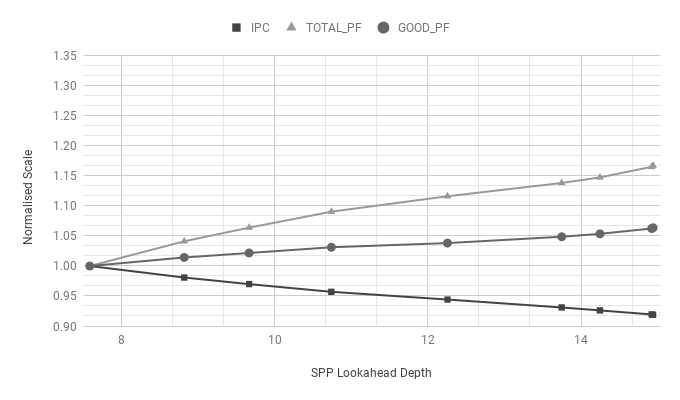
\includegraphics[width=\columnwidth]{Motivation}
\caption{The impact of aggressive prefetching on performance for {\tt 603.bwaves\_s}. 
The number of useful prefetches increases with aggressiveness
slower than total prefetches, which wastes bandwidth and 
harms performance.}
\label{Fig:Motivation}
\end{figure}

Coverage and accuracy are generally at odds with one another, and as
one metric improves, the other usually gets worse. For example, when
an application accesses a new region of memory for the first time, a
na\"ive prefetcher may predict that all data in that region will be
used by the application.  This will clearly result in 100\% coverage
for that region, but with possibly a very low accuracy.  In fact, so
much cache capacity and bandwidth may be wasted prefetching unused
data that performance can ultimately be harmed by this strategy. At
the other extreme, another prefetcher may be overly conservative and
never prefetch anything, wasting no capacity or bandwidth, and
achieving 0\% prefetch coverage.

Figure~\ref{Fig:Motivation} illustrates the above scenario.  Here we
consider a state-of-the-art. lookahead prefetcher -- SPP~\cite{SPP}.
Lookahead prefetchers such as SPP provide a mechanism to speculate an
arbitrary number of references ahead of the initial triggering miss.
In SPP, a throttling confidence threshold is then used to ensure that
the lookahead stops when confidence falls too low to ensure that
prefetches are accurate.  In the figure, we iteratively re-tuned 
this threshold to allow the prefetcher to lookahead a fixed
depth from 7 to 15. The figure depicts the behavior 
of the {\tt 603.bwaves\_s} SPEC CPU 2017 benchmark. The IPC, the 
total number of prefetches issued by the prefetcher (TOTAL\_PF), 
and the actual useful predictions (GOOD\_PF), all have been normalized 
to lookahead depth 7. As the lookahead
depth increases, so do useful prefetches, and hence coverage. This
coverage, however, comes at the cost of total prefetches increasing at
an even higher rate. This leads to cache pollution and bandwidth
contention, and leads to a reduction in IPC.  
%Similar behavior was observed in 12 other SPEC CPU 2017 benchmarks.

Therefore, a delicate balance between coverage and accuracy is
required for a prefetcher to maximize its performance impact.
Prefetchers are generally designed with internal mechanisms to monitor
their accuracy, and throttling mechanisms that can be tuned for either
coverage or accuracy.  The more irregular an application's memory
access pattern is, the more difficult it is to accurately predict
every access, so a prefetcher will have to be tuned more toward
coverage (and away from accuracy) in order to gain any benefit. This
may be especially dangerous to do in the context of a multi-core
processor, where overly aggressive prefetching in one core can waste
shared resources, such as last-level cache (LLC) capacity, and
off-chip bandwidth, impacting the performance of other
cores~\cite{Friendly}.

% Predicting future accesses requires a trade-off between coverage,
% the percent of predictions that prevented a cache miss, and
% accuracy, the percent of predictions made that were correct.
%% Gino: Just added a short explanation of coverage and accuracy
%% tradeoff, not sure if necessary
%A prefetcher may have high coverage by reducing the number of misses
% by simply requesting a large amount of data, however this does not
% imply accuracy. Even if the prefetcher brought in data accessed in
% the future, a high percentage of the data requested could never be
% accessed meaning the prefetcher had low accuracy, resulting in
% wasted resources as well as cache pollution. Likewise, a prefetcher
% can have a higher accuracy by being completely sure the data
% requested is used in the future, but may not affect performance
% since it did not have the coverage needed to make an
% impact. %end addition.
% Most prefetchers maintain an internal confidence mechanism by
% keeping counters to track events such as cache hits, misses,
% references to an entry in the prefetcher's structure, etc. By
% comparing the confidence indicated by the counters against different
% threshold values, the aggressiveness of the prefetcher can be
% adjusted, resulting in lower coverage and higher accuracy.

%For a prefetcher to capture highly irregular access patterns, it
% needs to be highly aggressive with high coverage. This causes the
% prefetcher to recommend many low accuracy prefetches that lead to
% the cache being polluted with useless data.  This effect is more
% pronounced in a multi-core scenario where the LLC is a shared
% resource~\cite{Friendly}. Conversely, a conservative prefetcher
% would be highly accurate but might not make enough useful prefetches
% due to its lower coverage.

Here, we propose Perceptron-based Prefetch Filtering (PPF) as an
enhancement to existing state-of-the-art prefetchers, allowing them to
speculate deeply to achieve high coverage while filtering out the
inaccurate prefetches this deep speculation implies.  PPF works by
observing the stream of candidate prefetches generated by a
prefetcher, and then rejects those that are predicted by the
online-trained neural model to be inaccurate.  The state-of-the-art
prefetcher that we use to evaluate PPF in this paper is the Signature
Path Prefetcher (SPP)~\cite{SPP}, however as we describe, PPF can be
designed to benefit any prefetcher.  In this design, PPF replaces
SPP's existing confidence-based throttling mechanism, which itself was
a highly tuned feature of that prefetcher.  Because PPF is so much
more effective at rejecting inaccurate prefetches than SPP's baseline
mechanism, we are free to re-tune the rest of SPP's design around
maximizing coverage. The result is an increase in both accuracy and
coverage, and a notable increase in performance.

%We propose Perceptron-based Prefetch Filtering (PPF) as an enhancement to
%the existing state of the art prefetchers to robustly overcome the coverage
%vs. accuracy trade-off. The idea is to use a state-of-the-art prefetcher as
%the base engine. For that we choose Signature Path Prefetcher (SPP) and
%modify the design to make it as aggressive as possible. This modification
%enables the base engine to capture complex memory access patterns and go
%deeper into the speculation path, increasing coverage without sacrificing accuracy. 
%Normally such aggressive prefetching would come at the cost of increased DRAM traffic
%and cache pollution. However, prefetch suggestions recommended by the base prefetch
%engine are passed through the perceptron based filter to ensure an accurate prediction.
%Over time, PPF learns to correlate the prefetch recommendations with various available
%features, leading to elimination of useless prefetches. This filtering leads
%to overall increased accuracy of the prefetch scheme and reduction in DRAM
%traffic and cache pollution.

This paper describes PPF, explains its merits, offers analysis, and
outlines the scope for future research. Its contributions are:

\begin{itemize}

\item An on-line neural model used for hardware data prefetching.
  Previous work in this area either relied on program
  semantics~\cite{Semantics} or were application
  specific~\cite{Datacenter}.

\item Implementing PPF filtering a state-of-the-art prefetcher, giving
  a significant performance improvement compared to previous work. PPF
  learns to adapt itself to shared resource constraints, leading to
  further increased performance in multi-core and
  bandwidth-constrained environments.

\item A methodology for determining an appropriate set of features for
  prediction, regardless of the underlying prefetcher used.  More
  details are explained in Section \ref{Method-Features}.

\end{itemize}

In a single core configuration, PPF increases performance by 3.78\%
compared to the underlying prefetcher, SPP. In a multi-core system running a
mixes of memory intensive SPEC CPU 2017 traces, PPF saw an improvement
of 11.4\% over SPP for a 4-core system, and 9.65\% for an 8-core system.

% djimenez - cutting this
%The paper is organized as follows. Section~\ref{Background} describes
%background work and summarizes SPP. Section~\ref{Arch} gives the 
%architectural overview of PPF. Section~\ref{Impl} discusses the
%implementation of PPF using SPP and the particular features used.
%Section~\ref{Method} gives the evaluation methodology and explores the feature
%space for perceptron learning. Section~\ref{Results} evaluates the
%performance of the prefetcher and Section~\ref{Conclusion} concludes the
%paper.
